\documentclass[12pt]{beamer}

\usetheme[sectionpage=none, subsectionpage=progressbar, progressbar=foot, numbering=fraction]{metropolis}

\makeatletter
\setlength{\metropolis@frametitle@padding}{1.6ex}% <- default 2.2 ex

\setbeamertemplate{footline}{%
  \begin{beamercolorbox}[wd=\textwidth, sep=1.5ex]{footline}% <- default 3ex
    \usebeamerfont{page number in head/foot}%
    \usebeamertemplate*{frame footer}
    \hfill%
    \usebeamertemplate*{frame numbering}
  \end{beamercolorbox}%
}
\makeatother

\AtBeginSubsection
{
  \begin{frame}{Where are we?}
    \tableofcontents[sectionstyle=show/shaded, subsectionstyle=show/shaded/hide]
  \end{frame}
}

\makeatletter
\setbeamertemplate{headline}{
  \begin{beamercolorbox}{upper separation line head}
  \end{beamercolorbox}
  \begin{beamercolorbox}{section in head/foot}
    \vskip2pt\insertsectionnavigationhorizontal{\paperwidth}{}{}\vskip2pt
  \end{beamercolorbox}
  \begin{beamercolorbox}{lower separation line head}
  \end{beamercolorbox}
}
\makeatother
\setbeamercolor{section in head/foot}{fg=normal text.bg, bg=structure.fg}

\setbeamertemplate{itemize items}[square]


\usepackage{menukeys}
\usepackage{minted}
\setminted[bash]{fontsize=\small, tabsize=2, breaklines}

\title{Hacker Tools: \\Shell \& Scripting}
\author{Julius Putra Tanu Setiaji}
\date{10 September 2019 \\ Slides at \url{https://is.gd/2019ht5slides}}

\begin{document}

\frame[plain]{\titlepage}

\section{Introduction}
\subsection{}

\begin{frame}{NUS Hackers}

  \begin{center}
    
\includegraphics[width=0.5\linewidth]{../NUSHackers}

    \url{http://nushackers.org}
  \end{center}

  \begin{center}
    \textbf{hacker}school

    Friday \textbf{Hacks}

    \textbf{Hack} \& Roll

    \textbf{Hacker} Tools
  \end{center}

\end{frame}

\begin{frame}{About Me}
  Hi! I'm Julius. My GitHub is \url{https://github.com/indocomsoft}

  A Year 3 Computer Science Undergraduate who loves hacking and building systems.

  I also enjoy Space Exploration, Music Theory and History.

    {\tiny (my favourite games are KSP and EU4 hit me up if you play those too)}
\end{frame}

\begin{frame}{What you will learn today}
  How to hack on a Unix-like environment:
  \begin{itemize}
    \item How to use the shell
    \item How to create scripts for automation
  \end{itemize}
\end{frame}

\begin{frame}{Required Software}
  Unix-like environment, either one of these:
  \begin{itemize}
    \item Linux (you're good if you attended and installed Linux during our Linux Install Fest last week)
    \item macOS\footnote{Open Terminal, and run \mintinline{bash}{xcode-select --install} first}
    \item BSD
    \item Other Unix-like OS'es (Minix, Solaris, AIX, HP-UX, etc.)
    \item WSL (Windows Subsystem for Linux) should also be alright, but no guarantee
  \end{itemize}
\end{frame}

\begin{frame}{Unix? Can I eat that?}
  \begin{itemize}
    \item A family of multitasking, multiuser OS'es.
    \item First developed in the 1970's.
    \item Popularised the use of interactive command line.
  \end{itemize}
  \begin{center}
    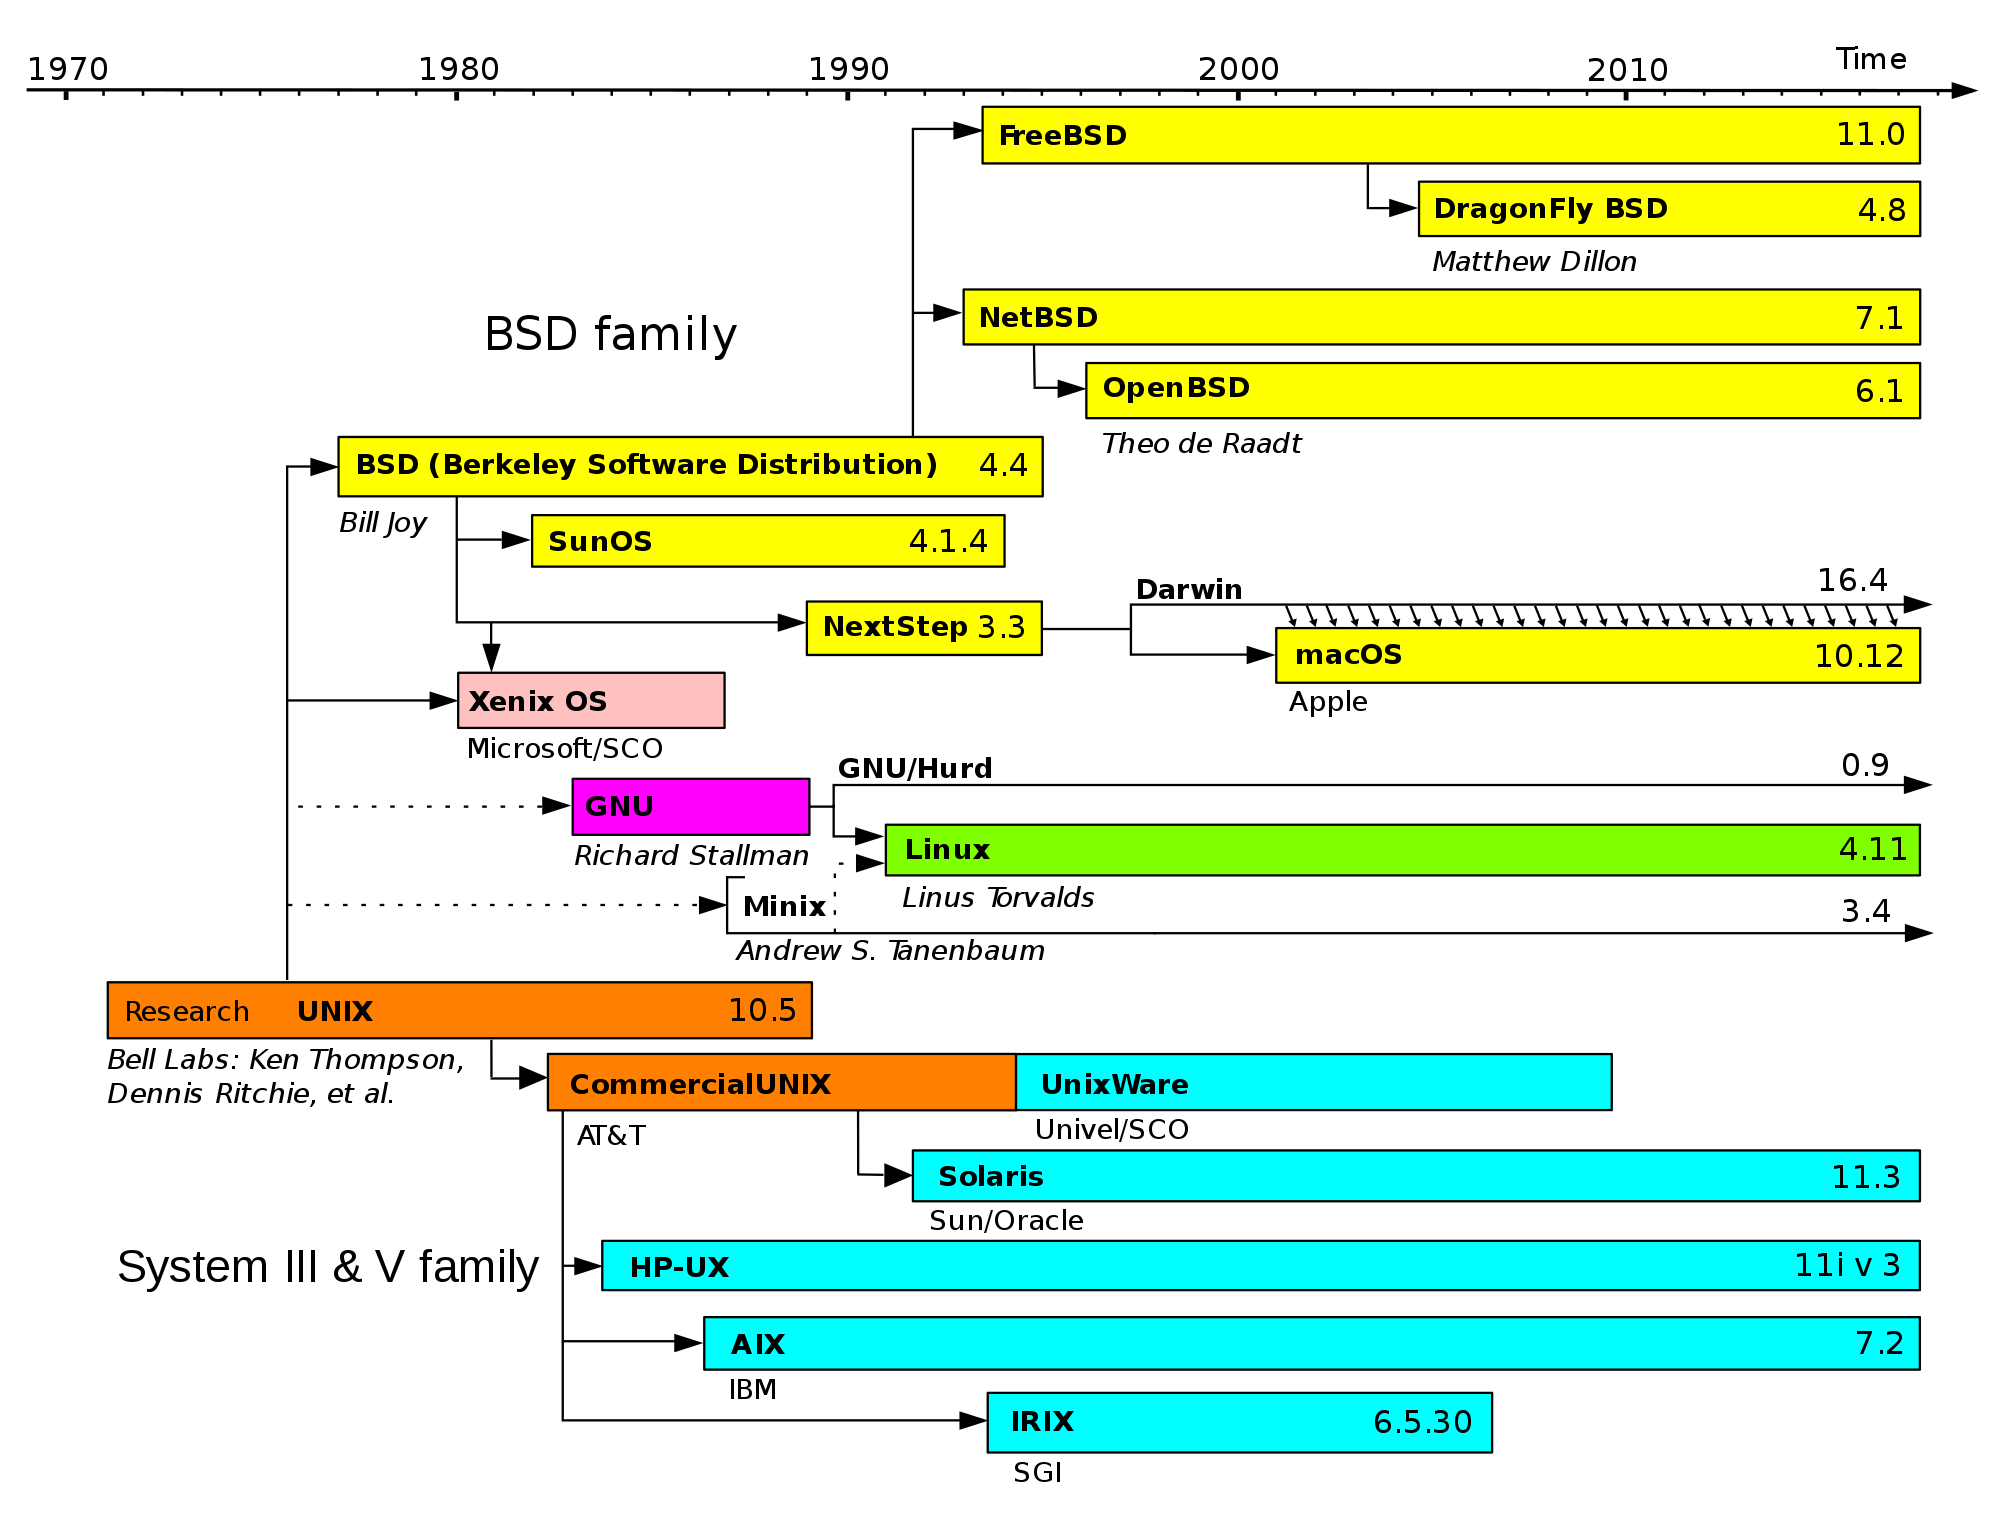
\includegraphics[width=0.6\linewidth]{unix_timeline}
  \end{center}
\end{frame}

\begin{frame}{The Unix Philosophy}
  \begin{enumerate}
    \item Write programs that do one thing and do it well.
    \item Write programs to work together.
    \item Write programs to handle text streams, because that is a universal interface.
  \end{enumerate}
\end{frame}

\section{Shell}
\subsection{}
\begin{frame}{Introduction to Shell}
  \begin{itemize}
    \item An efficient, textual interface to your computer.
    \item Provides an interactive programming language (``scripting'').
    \item Many shells to choose from:
          \begin{itemize}
            \item Standard ones: \texttt{sh} or \texttt{bash}
            \item Shells that match languages: \texttt{csh}
            \item "Better" shells: \texttt{fish}, \texttt{zsh}
          \end{itemize}
    \item For this workshop, the focus is on the ubiquitous \texttt{sh} and \texttt{bash}.\footnote{Feel free to explore other shells. On macOS, many people prefer \texttt{fish} or \texttt{zsh}}
  \end{itemize}
\end{frame}

\begin{frame}{The Shell Prompt}
  \begin{itemize}
    \item What greets you when you open a terminal.
          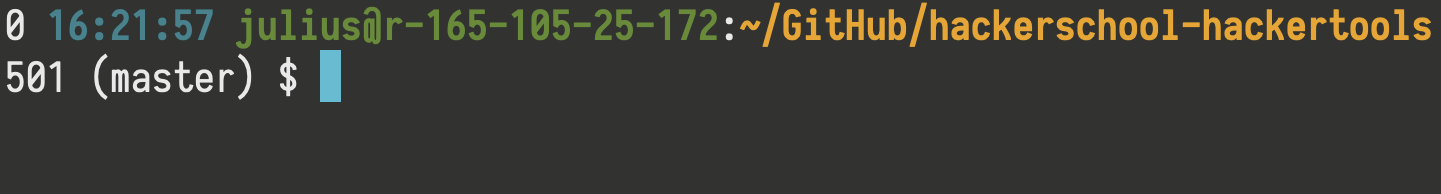
\includegraphics[width=\linewidth]{shell-prompt}
    \item Lets your run programmes and commands.
  \end{itemize}
\end{frame}

\begin{frame}{Common Commands}
  \begin{itemize}
    \item \mintinline{bash}{man} to get the \textbf{man}ual pages of a command
    \item \mintinline{bash}{cd} to \textbf{c}hange \textbf{d}irectory
    \item \mintinline{bash}{ls} to \textbf{l}i\textbf{s}t files and directories
    \item \mintinline{bash}{mkdir} to \textbf{m}a\textbf{k}e \textbf{dir}ectory
    \item \mintinline{bash}{rm} to \textbf{r}e\textbf{m}ove files and directories
    \item \mintinline{bash}{cp} to \textbf{c}o\textbf{p}y file
    \item \mintinline{bash}{mv} to \textbf{m}o\textbf{v}e file
  \end{itemize}
\end{frame}

\begin{frame}{Command Editing Shortcuts}
  \texttt{bash} has shortcuts based on \texttt{emacs} keybindings:
  \begin{itemize}
    \item \keys{\ctrlwin + a}: beginning of line
    \item \keys{\ctrlwin + e}: end of line
    \item \keys{\Altwin + b}: move back one word
    \item \keys{\Altwin + f}: move forward one word
    \item \keys{\ctrlwin + k}: delete from cursor to the end of line
  \end{itemize}
  And some special ones:
  \begin{itemize}
    \item \keys{\ctrlwin + u}: delete from cursor to the start of line
    \item \keys{\ctrlwin + w}: delete from cursor to start of word
  \end{itemize}
\end{frame}

\begin{frame}{Command Control Shortcuts}
  \begin{itemize}
    \item \keys{\ctrlwin + c}: terminates the command
    \item \keys{\ctrlwin + z}: suspends the command (\mintinline{bash}{fg} to continue)
    \item \keys{\ctrlwin + l}: clears the screen
    \item \keys{\ctrlwin + s}: stops the output to the screen
    \item \keys{\ctrlwin + q}: allows output to the screen
  \end{itemize}
\end{frame}

\section{Scripting}
\subsection{Introduction}

\begin{frame}[fragile]{Script (1/2)}
  You can write programs directly at the prompt, or write into a file (writing scripts)
  \begin{minted}[linenos]{bash}
#!/bin/sh
echo something
\end{minted}
  \begin{itemize}
    \item Open an editor (for beginner, \mintinline{bash}{nano} is recommended), save the script as \texttt{example-script}
    \item On your shell, run \mintinline{bash}{chmod +x example-script}
    \item You can run your script as \mintinline{bash}{./example-script}
  \end{itemize}
\end{frame}

\begin{frame}[fragile]{Script (2/2)}
  \begin{minted}[linenos]{bash}
#!/bin/sh
echo something
\end{minted}
  Magic?
  \begin{itemize}
    \newsavebox\mybox
    \begin{lrbox}{\mybox}
      {\scriptsize\mintinline{bash}{#!/usr/bin/env python}}
    \end{lrbox}
    \item \mintinline{bash}{#!/bin/sh} is also known as the \textbf{shebang}, specifies the interpreter\footnote{You can use other interpreters too, e.g. \footnotesize\usebox{\mybox} for a python script.}
    \item \mintinline{bash}{echo} is a command that prints its arguments to the standard output.
  \end{itemize}
\end{frame}

\begin{frame}[fragile]{Flags (1/3)}
  \begin{itemize}
    \item Most command line utilities take parameters using \textbf{flags}.
    \item They come in short form (\texttt{-h}) and long form (\texttt{--help})
    \item Usually, running \mintinline{bash}{COMMAND -h} or \mintinline{bash}{man COMMAND} will give you a list of the flags the program takes.
    \item Short flags can be combined: \mintinline{bash}{rm -r -f} is equivalent to \mintinline{bash}{rm -rf} or \mintinline{bash}{rm -fr}
  \end{itemize}
\end{frame}

\begin{frame}[fragile]{Flags (2/3)}
  \begin{itemize}
    \item A double dash \texttt{--} is used in to signify the end of command options, after which only positional parameters are accepted.
          \begin{itemize}
            \item For example, to create a file called \texttt{-v}, Use \mintinline{bash}{touch -- -v} instead of \mintinline{bash}{touch -v}
            \item For example, to grep a file called \texttt{-v}, \mintinline{bash}{grep pattern -- -v} will work while \mintinline{bash}{grep pattern -v} will not.
          \end{itemize}
  \end{itemize}
\end{frame}

\begin{frame}[fragile]{Flags (3/3)}
  Some common flags are a de facto standard:
  \begin{itemize}
    \item \texttt{-a} commonly refers to all files (i.e. also including those that start with a period\footnote{In Unix, by convention files whose names begin with a period is hidden})
    \item \texttt{-f} usually refers to forcing something, e.g. \mintinline{bash}{rm -f}
    \item \texttt{-h} displays the help for most commands
    \item \texttt{-v} usually enables a verbose output
    \item \texttt{-V} usually prints the version of the command
  \end{itemize}
\end{frame}

\begin{frame}{Unix Directory Structure}
  Unix has a different directory structure from Windows.

  There is no concept of drives.

  Everything is files and directories. The root directory is \texttt{/}

  We use forward slash \texttt{/} instead of backward slash \texttt{\textbackslash}

  Specifically for Linux, there is FHS\footnote{\url{https://en.wikipedia.org/wiki/Filesystem_Hierarchy_Standard}}
\end{frame}

\begin{frame}{Important Unix Directories}
  \begin{itemize}
    \item \texttt{/bin}, \texttt{/sbin}, \texttt{/usr/bin}, \texttt{/usr/local/bin}, \texttt{/opt} = executables
    \item On Linux: \texttt{/home} = user home directories
    \item On macOS: \texttt{/Users} = user home directories
    \item \texttt{/var/log} = log files
    \item \texttt{/tmp} = temporary files
  \end{itemize}
\end{frame}

\subsection{Shell Syntax}
\begin{frame}[fragile]{Running a command}
  \begin{minted}{bash}
echo Hello
\end{minted}
  \begin{itemize}
    \item \mintinline{bash}{COMMAND ARG1 ARG2 ARG3}
  \end{itemize}
\end{frame}

\begin{frame}[fragile]{Variables (1/3)}
  \begin{minted}{bash}
echo location
name=Julius
echo $name
\end{minted}
  \begin{itemize}
    \item Used to store text
    \item \mintinline{bash}{name=value} to set variable
    \item \mintinline{bash}{$name} to access variable %$
  \end{itemize}
\end{frame}

\begin{frame}[fragile]{Variables (2/3)}
  There are also a number of special variables:
  \begin{itemize}
    \item \mintinline{bash}{$?}: get exit code of the previous command %$
    \item \mintinline{bash}{$1} to \mintinline{bash}{$9}: arguments to a script %$
    \item \mintinline{bash}{$0}: name of the script itself %$
    \item \mintinline{bash}{$#}: number of arguments %$
    \item \mintinline{bash}{$$}: process ID of current shell %$

  \end{itemize}
\end{frame}

\begin{frame}[fragile]{Variables (3/3)}
  Create a script \texttt{variable-example} containing the code below, then try running it with various arguments.
  \begin{minted}[linenos]{bash}
#!/bin/sh
echo $0
echo $1
echo $2
echo $#
\end{minted}

\end{frame}

\begin{frame}[fragile]{Loop (1/4)}
  Loop is used to run a command a bunch of times.

  For example:
  \begin{minted}{bash}
for i in $(seq 1 5); do echo hello; done
\end{minted}
\end{frame}

\begin{frame}[fragile]{Loop (2/4)}
  \begin{minted}{bash}
for i in $(seq 1 5); do echo hello; done
\end{minted}
  Let's unpack this!

  \mintinline{bash}{for x in list; do BODY; done}
  \begin{itemize}
    \item \mintinline{bash}{;} terminates a command -- equivalent to newline
    \item Split \mintinline{bash}{list}, assign each to \mintinline{bash}{x}, and run \mintinline{bash}{BODY}
    \item Split by ``whitespace'' -- we will get into it later
    \item Compared to C, no curly braces, instead \mintinline{bash}{do} and \mintinline{bash}{done}
  \end{itemize}
\end{frame}


\begin{frame}[fragile]{Loop (3/4)}
  \begin{minted}{bash}
for i in $(seq 1 5); do echo hello; done
\end{minted}
  Let's unpack this!

  \mintinline{bash}{$(seq 1 5)} %$
  \begin{itemize}
    \item Run the program \mintinline{bash}{seq} with arguments \texttt{1} and \texttt{5}
    \item Substitute the \mintinline{bash}{$(...)} block with the output of the program %$
    \item Equivalent to
          \begin{minted}{bash}
for i in 1 2 3 4 5; do echo hello; done
  \end{minted}
  \end{itemize}
\end{frame}

\begin{frame}[fragile]{Loop (4/4)}
  \begin{minted}{bash}
for i in $(seq 1 5); do echo hello; done
\end{minted}
  Let's unpack this!

  \mintinline{bash}{echo hello}
  \begin{itemize}
    \item Everything in a shell script is a command
    \item Here, it means run the \mintinline{bash}{echo} command, with argument \texttt{hello}.
    \item All commands are searched in \mintinline{bash}{$PATH} (colon-separated) %$
    \item Find out where a command is located by running \mintinline{bash}{which COMMAND}, e.g. \mintinline{bash}{which ls}
  \end{itemize}
\end{frame}

\begin{frame}[fragile]{Conditionals (1/2)}
  \begin{minted}{bash}
if test -d /bin; then echo true; else echo false; fi;
\end{minted}
  Let's unpack this!

  \mintinline{bash}{if CONDITION; then BODY; fi}
  \begin{itemize}
    \item \mintinline{bash}{CONDITION} is a command.
    \item If its exit code is \texttt{0} (success), then \mintinline{bash}{BODY} is run.
    \item Optionally, you can also hook in an \mintinline{bash}{else} or \mintinline{bash}{elif}
  \end{itemize}
\end{frame}

\begin{frame}[fragile]{Conditionals (2/2)}
  \begin{minted}{bash}
if test -d /bin; then echo true; else echo false; fi;
\end{minted}
  Let's unpack this!

  \mintinline{bash}{test -d /bin}
  \begin{itemize}
    \item \mintinline{bash}{test} is a program that provides various checks and comparison which exits with exit code \texttt{0} if the condition is true\footnote{Remember, you can check exit code using \mintinline{bash}{$?}}. %$
    \item Alternate syntax: \mintinline{bash}{[ condition ]}, e.g. \mintinline{bash}{[ -d /bin ]}
  \end{itemize}
\end{frame}

\begin{frame}[fragile]{Everything Together}
  Let's create a command like \mintinline{bash}{ls} that only prints directories:
  \begin{minted}[linenos]{bash}
#!/bin/sh
for f in $(ls)
do
  if test -d $f
  then
    echo dir $f
  fi
done
\end{minted}
\end{frame}

\begin{frame}{Bug!}
  Hold on! What if the directory is called "\texttt{My Documents}"?
  \begin{itemize}
    \item \mintinline{bash}{for f in $(ls)} expands to \\\mintinline{bash}{for f in My Documents} %$
    \item Will first perform the test on \texttt{My}, then on \texttt{Documents}
    \item Not what we wanted!
  \end{itemize}
\end{frame}

\begin{frame}{Argument Splitting}
  \begin{itemize}
    \item Bash splits arguments by whitespace (tab, newline, space)
    \item Same problem somewhere else: \mintinline{bash}{test -d $f} %$
    \item If \mintinline{bash}{$f} contains whitespace, \mintinline{bash}{test} will error! %$
    \item Need to use quote to handle spaces in arguments \mintinline{bash}{for f in "My Documents"}
    \item How do we fix our script?
    \item What do you think \mintinline{bash}{for f in "$(ls)"} does? %$
  \end{itemize}
\end{frame}

\begin{frame}[fragile]{Globbing (1/2)}
  \begin{itemize}
    \item \mintinline{bash}{bash} knows how to look for files using patterns:
          \begin{itemize}
            \item \mintinline{bash}{*}: any string of characters
            \item \mintinline{bash}{?}: any single character
            \item \mintinline{bash}{{a,b,c}}: any of these characters
          \end{itemize}
    \item Thus, \mintinline{bash}{for f in *} means all files in this directory
    \item When globbing, each matching file becomes its own argument
    \item However, still need to make sure to quote, e.g.\\ \mintinline{bash}{test -d "$f"} %$
  \end{itemize}
\end{frame}

\begin{frame}[fragile]{Globbing (2/2)}
  You can make advanced patterns
  \begin{itemize}
    \item \mintinline{bash}{for f in a*}: \pause all files starting with \texttt{a} in the current directory
    \item \mintinline{bash}{for f in foo/*.txt}: \pause all \texttt{.txt} files in \texttt{foo}
    \item \mintinline{bash}{for f in foo/*/p??.txt}: \pause all three-letter text files, starting with p, in subdirectories of \texttt{foo}
  \end{itemize}
\end{frame}

\begin{frame}{Other whitespace issues}
  \begin{itemize}
    \item \mintinline{bash}{if [ $foo = "bar" ]; then}: What's the issue? %$
          \pause
    \item What if \mintinline{bash}{$foo} is empty? arguments to \mintinline{bash}{[} are \texttt{=} and \texttt{bar} %$
    \item Possible workaround: \mintinline{bash}{[ x$foo = "xbar" ]}, but very hacky %$
          \pause
    \item Instead, use \mintinline{bash}{[[ CONDITION ]]}: \texttt{bash} built-in comparator that has special parsing
    \item Good news: it also allows \mintinline{bash}{&&} instead of \mintinline{bash}{-a}, \mintinline{bash}{||} instead of \mintinline{bash}{-o}, etc.
  \end{itemize}
\end{frame}

\begin{frame}{shellcheck}
  \begin{itemize}
    \item The mentioned problems are the most common bugs in shell scripts.
    \item A good tool to check for these kinds of possible bugs in your shell script: \url{https://www.shellcheck.net/}
  \end{itemize}
\end{frame}

\subsection{Composability}
\begin{frame}{Composability}
  \begin{itemize}
    \item Shell is powerful, in part because of \textbf{Composability}
    \item You can chain multiple programs together, rather than one program that does everything
    \item Remember \textbf{The Unix Philosophy}:
          \begin{enumerate}
            \item Write programs that do one thing and do it well.
            \item Write programs to work together.
            \item Write programs to handle text streams, because that is a universal interface.
          \end{enumerate}
  \end{itemize}
\end{frame}

\begin{frame}[fragile]{Pipe (1/2)}
  \begin{minted}{bash}
dmesg | tail
  \end{minted}
  Let's unpack this!

  \mintinline{bash}{a | b}
  \begin{itemize}
    \item Means run both \texttt{a} and \texttt{b}, but send all the output of \texttt{a} as input to \texttt{b}, and then print the output of \texttt{b}
  \end{itemize}
\end{frame}

\begin{frame}[fragile]{Pipe (2/2)}
  You can chain this even longer!

  \mintinline{bash}{cat /var/log/sys*log | grep Sep 10 | tail}
  \begin{itemize}
    \item \mintinline{bash}{cat /var/log/sys*log} prints the system log
    \item This output is fed into \mintinline{bash}{grep Sep 10}, which looks for all entries from today.
    \item This output is then further fed into \mintinline{bash}{tail}, which prints only the last 10 lines.
  \end{itemize}
\end{frame}

\begin{frame}[fragile]{Streams}
  \begin{itemize}
    \item All programs launched have 3 streams:
          \begin{itemize}
            \item \texttt{STDIN}: the program reads input from here
            \item \texttt{STDOUT}: the program prints to here
            \item \texttt{STDERR}: a second output that the program can choose to use.
          \end{itemize}
    \item By default, \texttt{STDIN} is your keyboard, \texttt{STDOUT} and \texttt{STDERR} are both your terminal
  \end{itemize}
\end{frame}

\begin{frame}[fragile]{Stream Redirection (1/2)}
  \begin{itemize}
    \item However, this can be changed!
    \item \mintinline{bash}{a | b}: makes \texttt{STDOUT} of \texttt{a} the \texttt{STDIN} of \texttt{b}.
    \item \mintinline{bash}{a > foo}: \texttt{STDOUT} of \texttt{a} goes to the file \texttt{foo}
    \item \mintinline{bash}{a 2> foo}: \texttt{STDERR} of \texttt{a} goes to the file \texttt{foo}
    \item \mintinline{bash}{a < foo}: \texttt{STDIN} of \texttt{a} is read from the file \texttt{foo}
    \item \mintinline{bash}{a <<< some text}: \texttt{STDIN} of \texttt{a} is read from what comes after \texttt{<<<}
    \item You can also pipe to \texttt{tee} (look up in \texttt{man} what \texttt{tee} does)
  \end{itemize}
\end{frame}

\begin{frame}[fragile]{Stream Redirection (2/2)}
  \textbf{So why is this useful?} \pause

  It lets you manipulate output of a program!
  \pause
  \begin{itemize}
    \item \mintinline{bash}{ls | grep foo}: all files that contain the word \texttt{foo}
    \item \mintinline{bash}{ps | grep foo}: all processes that contain the word \texttt{foo}
    \item On Linux: \mintinline{bash}{journalctl | grep -i intel | tail -n 5}: last 5 system log messages with the word \texttt{intel} (case-insensitive)
    \item Note that this forms the basis for \textbf{data-wrangling}, which will be covered later.
  \end{itemize}
\end{frame}

\begin{frame}[fragile]{Grouping Commands}
  \mintinline{bash}{(a; b) | tac}
  \begin{itemize}
    \item Run \texttt{a}, then \texttt{b}, and send all their output to \texttt{tac}\footnote{\texttt{tac} print in reverse}
    \item For example: \mintinline{bash}{(echo qwe; echo asd; echo zxc) | tac}
  \end{itemize}
\end{frame}

\begin{frame}[fragile]{Process Substitution}
  \mintinline{bash}{b <(a)}
  \begin{itemize}
    \item Run \texttt{a}, generate a temporary file name for its output stream, and pass that filename to \texttt{b}
    \item To demonstrate: \mintinline{bash}{echo <(echo a) <(echo b)}
    \item On Linux: \mintinline{bash}{diff <(journalctl -b -1 | head -n20) <(journalctl -b -2 | head -n20)}
    \item This shows the difference between the first 20 lines of the last boot log and the one before that.
  \end{itemize}
\end{frame}

\subsection{Job and Process Control}
\begin{frame}[fragile]{Job (1/2)}
  Used to run longer-term things in the background.
  \begin{itemize}
    \item Use the \mintinline{bash}{&} suffix
          \begin{itemize}
            \item It will give back your prompt immediately.
            \item For example: \mintinline{bash}{(for i in $(seq 1 100); do echo hi; sleep 1; done) &}
            \item Note that the running program still has your terminal as \texttt{STDOUT}. Instead, can redirect \texttt{STDOUT} to file.
            \item Handy especially to run 2 programs at the same time like a server and client: \mintinline{bash}{server & client}
            \item For example: \mintinline{bash}{nc -l 1234 & nc localhost 1234 <<< test}
          \end{itemize}
  \end{itemize}
\end{frame}

\begin{frame}[fragile]{Job (2/2)}
  \begin{itemize}
    \item \mintinline{bash}{jobs}: see all jobs
    \item \mintinline{bash}{fg %JOBS}: bring the job corresponding to the id to the foreground (with no argument, bring the latest job to foreground)
    \item You can also background the current program: \texttt{\^{}Z}\footnote{\keys{\ctrlwin} is usually denoted as \^{}, thus \keys{\ctrlwin + z} is denoted as \texttt{\^{}Z}}, then run \mintinline{bash}{bg}
          \begin{itemize}
            \item \texttt{\^{}Z} stops the current process and makes it a job.
            \item \mintinline{bash}{bg} runs the last job in the background.
          \end{itemize}
    \item \mintinline{bash}{$!} is the PID of the last background process.
  \end{itemize}
\end{frame}

\begin{frame}[fragile]{Process Control (1/2)}
  \begin{itemize}
    \item \mintinline{bash}{ps}: lists running processes
          \begin{itemize}
            \item \mintinline{bash}{ps -A}: lists processes from all users
            \item Check out the man page for other arguments.
          \end{itemize}
    \item \mintinline{bash}{pgrep}: find processes by searching (like \mintinline{bash}{ps -A | grep})
          \begin{itemize}
            \item \mintinline{bash}{pgrep -f}: find processes with arguments
          \end{itemize}
    \item \mintinline{bash}{kill}: send a \emph{signal} to a process by ID (\mintinline{bash}{pkill} to search and run \mintinline{bash}{kill})
          \begin{itemize}
            \item Signal tells a process to do something
            \item \texttt{SIGKILL} (\texttt{-9} or \texttt{-KILL}): tell it to exit \emph{right now} (equivalent to \texttt{\^{}\textbackslash})
            \item \texttt{SIGTERM} (\texttt{-15} or \texttt{-TERM}): tell it to exit gracefully (equivalent to \texttt{\^{}C})
          \end{itemize}
  \end{itemize}
\end{frame}

\begin{frame}[fragile]{Process Control (2/2)}
  \begin{itemize}
    \item \mintinline{bash}{kill}: send a \emph{signal} to a process by ID (\mintinline{bash}{pkill} to search and run \mintinline{bash}{kill})
          \begin{itemize}
            \item Signal tells a process to do something
            \item Most common\footnote{Prefer \texttt{SIGTERM} over \texttt{SIGKILL}: \url{https://turnoff.us/geek/dont-sigkill/}}:
                  \begin{itemize}
                    \item \texttt{SIGKILL} (\texttt{-9} or \texttt{-KILL}): tell it to exit \emph{right now} (equivalent to \texttt{\^{}\textbackslash})
                    \item \texttt{SIGTERM} (\texttt{-15} or \texttt{-TERM}): tell it to exit gracefully (equivalent to \texttt{\^{}C})
                  \end{itemize}
          \end{itemize}
  \end{itemize}
\end{frame}

\begin{frame}{More Resources}
  \begin{itemize}
    \item If you are completely new to the shell, you might want to read a comprehensive guide, such as BashGuide\footnote{\url{http://mywiki.wooledge.org/BashGuide}}.
    \item For a more in-depth introduction, The Linux Command Line\footnote{\url{http://linuxcommand.org/tlcl.php}} is a good resource.
  \end{itemize}
\end{frame}

\subsection{Exercises}
\begin{frame}{xargs}
  \begin{itemize}
    \item Sometimes piping doesn't quite work because the command being piped into does not expect the newline separated format.
    \item For example, \texttt{file} command tells you properties of the file.
    \item Try running \mintinline{bash}{ls | file} and \mintinline{bash}{ls | xargs file}
    \item What is \mintinline{bash}{xargs} doing?
  \end{itemize}
\end{frame}

\begin{frame}{Other Exercises}
  \begin{itemize}
    \item Try running \mintinline{bash}{touch {a,b}{a,b}}, then \mintinline{bash}{ls}. What appeared?
    \item Sometimes you want to keep \texttt{STDIN} and still output to a file. Try running \mintinline{bash}{echo HELLO | tee hello.txt}
    \item Run \mintinline{bash}{echo HELLO > hello.txt}, then \mintinline{bash}{echo WORLD >> hello.txt}. What are the contents of \texttt{hello.txt}? How is \mintinline{bash}{>} different from \mintinline{bash}{>>}?
  \end{itemize}
\end{frame}

\section{Conclusion}
\subsection{}
\begin{frame}
  \frametitle{Talk to us!}
  \begin{itemize}
    \item \textbf{Feedback form}: \url{https://is.gd/2019ht5}
    \item \textbf{Upcoming Hacker Tools}:

          Data Wrangling, SR1, 17th September 2019, 7pm
  \end{itemize}
\end{frame}

\end{document}
